\documentclass[9pt]{article}
\usepackage{graphicx}
\usepackage{float}
\usepackage[T1]{fontenc}
\usepackage{helvet}
\renewcommand{\familydefault}{\sfdefault}
\renewcommand{\quad}{\hspace{0.5cm}}
\linespread{1.5}
\usepackage[margin=1in]{geometry}

\begin{document}

Pedro Francisco Sousa e Silva PG50689, Tiago Aguiar Martins PG50775 e Dong Xuyong PG50343 (TP2 Grupo 5).

\section{Introdução}

\quad Within the subject of Artificial Intelligence Techniques in Forecasting and Optimization in Business Systems, we were proposed a project aimed at using forecasting and optimization techniques in a real mind problem, in this case the distribution of drinks in a company.

Throughout this document we will first analyze the beverage sales data, then we will apply forecasting techniques to predict the number of sales of each beverage, this forecast will be divided by a univariate forecast and a multivariate forecast, for both will be used the knowledge and practices acquired in class to predict successfully. Finally, we have Optimization, which consists of finding the best values in order to maximize the sales value of each drink.

\section{Dataset and Requirements}


\quad For this project, we were provided with an excel file called "bebidas.xlsx", within which are the daily sales records of each of the two beverages made available by the company in question, within that excel file there are still other relevant data, which will be detailed afterwards.

\subsection{Parametros do dataset}


\quad In the following image we have a print of the columns of the dataset mentioned above:

\begin{figure}[H]
    \centering
    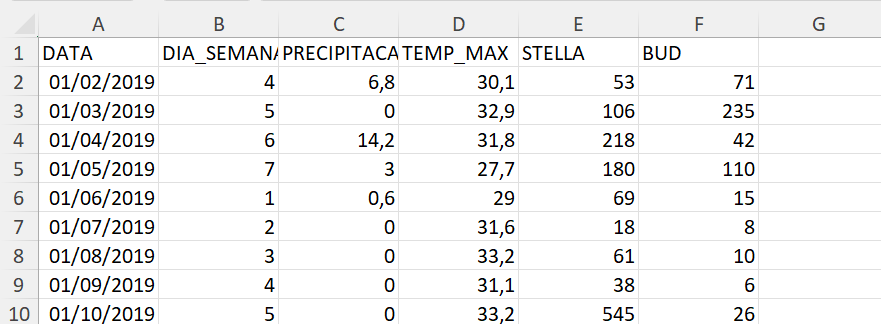
\includegraphics[width=0.8\textwidth]{assets/dataset.png}
    \caption{Project Dataset}
    \label{fig:dataset}
    \end{figure}

\quad The following dataset is compose of 6 columns, they being:

\quad \quad \textbullet DATA: This column represents the date the records are from;

\quad \quad \textbullet DIA\_SEMANA: This column represents the day of the week, where 1 is Sunday, 2 is Monday, 3 is Tuesday, 4 is Wednesday, 5 is Thursday, 6 is Friday and 7 is Saturday;

\quad \quad \textbullet PRECIPITACAO: This column represents the total of precipitation in mm in that day;

\quad \quad \textbullet TEMP\_MAX: This column represents the daily maximum temperature in Celcius from that day;

\quad \quad \textbullet STELLA: This column represents the number of STELLA drinks that where sold in that day;

\quad \quad \textbullet BUD: This column represents the number of BUD drinks that where sold in that day.

\subsection{Graficos}


semanasxvendas

autocorrelation plot
\subsection{Requisitos}

entender o negócio
\section{Previsão}

\quad Now that we have a good idea of the problem in questian and all the data related to that problem, now we shall start to use Machine Lerning techniques to predict the values of the next day using all the data from the data in the excel file. 

There are two way we can predict the values, using only one set of values, Univariate Search, or we can use more than one set of values, Multivariate Search. In this section of the document we will demonstrate the techniques used to predict and the respective results.

\subsection{Univariados}

\quad For the Univariate Search we use two methods of predction, prediction using split and prediction using growing and rowling window.

\subsubsection{Univariados Split}


\quad For the Split method first we split the number of occurences in two pieces, training set and test set, in our case it was a split of 80/20, that is 80\% training and 20\% test.

After that we used predictions techniques from the libraries rminer and forecast and we arrived at this conclusions:
\subsubsection{Rowling and Growing Windows}


\quad For the Growin/Rowling Window methods consists in doing the split in windows, for our exemple we used windows of the size 7, that where meant to indicate 7 days, one week.

After that we used predictions techniques from the libraries rminer and forecast and we arrived at this conclusions:
\subsection{Multivariados}

\subsubsection{Multivariados Split}
\section{Optimização}

\end{document}